\lipsum[1] % Texte de remplissage pour donner un exemple de la mise en page

% Exemple de déclaration de figure
\begin{figure}
	\centering % Les figures doivent être centrées
	\fbox{ % Les figures doivent être délimitées par un rectangle
		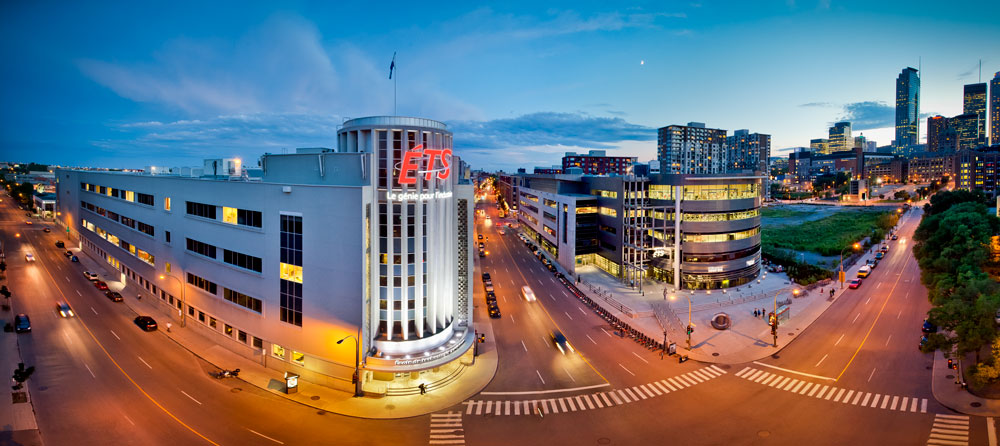
\includegraphics[width=0.75\textwidth]{figures/vueEts.jpg} % Spécification du paramètres "width", la largeur de l'image (en conservant les proportions). La largeur est ici restreinte à 0.75 fois "\textwidth", qui est la largeur maximale du texte dans le document en prenant en compte les marges
	}
	 \\ \parbox{0.75\textwidth}{\caption{Test de longue légende, avec utilisation de framebox et parbox pour restreindre la largeur de la légende.}\label{fig:vueEts}} % Utilisation d'une parbox pour restreindre la largeur de la légende. Ici la taille maximale a été fixée à la largeur choisie pour l'image (0.75\textwidth). Le décanat demande d'éviter d'avoir des légendes qui dépasse les figures, dans la mesure du possible (si l'image est trop petite, la légende peut dépasser sa largeur).
\end{figure}

\lipsum[1] % Texte de remplissage pour donner un exemple de la mise en page